\documentclass[14pt]{beamer}
\usepackage{fontspec}
\usepackage{color}
\usepackage{minted}

%% These fonts are non-free.
%% Comment out the lines if you don't have them.
\setmainfont{Equity Text A}
\setsansfont{Concourse T3}
\setmonofont{Triplicate T4}

\definecolor{bgcolor}{RGB}{20,25,28}
\setbeamercolor{background canvas}{bg=bgcolor}
\setbeamercolor{normal text}{fg=white}
\setbeamercolor{itemize item}{fg=white}
\setbeamertemplate{itemize items}[circle]
%% These styles are kinda annoying the fuck outta me
%% If I have a change of heart (again), then here's the
%% file to edit:
%% /usr/lib/python3.6/site-packages/pygments/styles/monokai.py
%% Don't forget to remove the _minted* dir afterwards.
\usemintedstyle[common-lisp]{monokai}

\renewcommand{\theFancyVerbLine}{\color{darkgray}\large \oldstylenums{\arabic{FancyVerbLine}}}
\newcommand{\toptitle}[1]{
  {\huge #1} \\
  \vspace{0.2cm}
}
\renewcommand{\subtitle}[1]{
  {\large #1} \\
  \vspace{0.2cm}
}
\newminted[lispcode]{common-lisp}{fontsize=\footnotesize}

\begin{document}
\begin{frame}
  \begin{center}
    
\includegraphics[height=4cm]{avatar.png}\\
    \vspace{0.2cm}
    {\Large Nicolas Hafner} \\
    \vspace{0.2cm}
    {\LARGE @Shinmera} \\
    \vspace{0.2cm}
    \url{https://everything.shinmera.com}
  \end{center}
\end{frame}

\begin{frame}
  \toptitle{Web Frameworks}
  \begin{itemize}
  \item HTTP Server
  \item Database
  \item Handling of common problems
  \item Template rendering
  \item User accounts, authentication
    \pause
  \item Potentially everything in computing too
  \end{itemize}
\end{frame}

\begin{frame}
  \toptitle{About Seven Years Ago}
  \begin{center}
    
\includegraphics[width=0.8\columnwidth]{baby-at-computer.jpg}
  \end{center}
\end{frame}

\begin{frame}
  \toptitle{About Seven Years Ago}
  \begin{itemize}
  \item Comics with comments
  \item Forums for discussions
  \item How not to require users to have multiple logins?
    \pause
  \item Write my own software \pause ... in PHP
  \item Evolved over time, eventually I got to Lisp
  \end{itemize}
\end{frame}

\begin{frame}
  \toptitle{Radiance Goals}
  \begin{itemize}
  \item ``Do it right this time''
  \item Run multiple applications side-by-side
  \item Share resources between applications
  \item Make as many parts optional as possible
  \item Configurable by administrator
  \item Documented well and easy to use
  \end{itemize}
\end{frame}

\begin{frame}
  \toptitle{Interfaces}
  \begin{itemize}
  \item Standardise access to common features
  \item Load interface implementation on demand
  \item Weak contract to ensure consistency
  \end{itemize}
\end{frame}

\begin{frame}[fragile]
  \toptitle{Interface Definition}
\begin{lispcode}
(define-interface cache
  (defun invalidate (name)
    "Causes the cached value to be re-computed.")

  (defmacro with-caching (name test &body body)
    "Caches the return value if TEST is non-NIL."))
\end{lispcode}
\end{frame}

\begin{frame}[fragile]
  \toptitle{Interface Implementation}
\begin{lispcode}
(defvar cache::*caches* (make-hash-table))

(defun cache:invalidate (name)
  (remhash name *caches*))

(defmacro cache:with-caching (name test &body body)
  (once-only (name)
    `(or (and (not ,test) (gethash ,name *caches*))
         (setf (gethash ,name *caches*)
               (progn ,@body)))))
\end{lispcode}
\end{frame}

\begin{frame}[fragile]
  \toptitle{Interface Usage}
\begin{lispcode}
(asdf:defsystem another-todo-app
  ...
  :depends-on ((:interface :cache)))

...

(in-package :another-todo-app)

(defun render-todo-list (user)
  (cache:with-caching (user (changes-made-p user))
    (render-template (template "todo-list.html")
                     (fetch-todo-items user))))
\end{lispcode}
\end{frame}

\begin{frame}
  \toptitle{Interface Advantages}
  \begin{itemize}
  \item No overhead as everything is direct calls
  \item Supports all kinds of definitions
  \item Allows framework to grow or shrink as needed
  \item Implementation can be exchanged
  \end{itemize}
\end{frame}

\begin{frame}
  \toptitle{Routing}
  \begin{itemize}
  \item Find proper content to deliver on an address
  \item Share the address space between applications
  \item Make it easy to visualise and understand
  \end{itemize}
\end{frame}

\begin{frame}
  \toptitle{Routing Life-Cycle}
  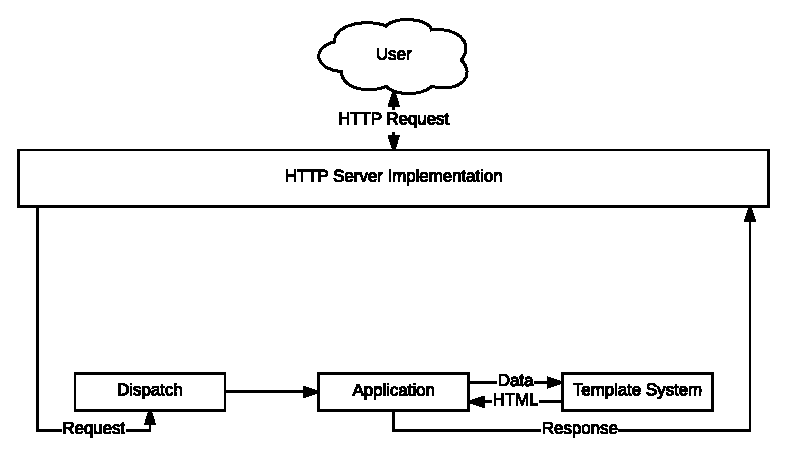
\includegraphics[width=\columnwidth]{request-simple}
\end{frame}

\begin{frame}
  \toptitle{Routing Life-Cycle}
  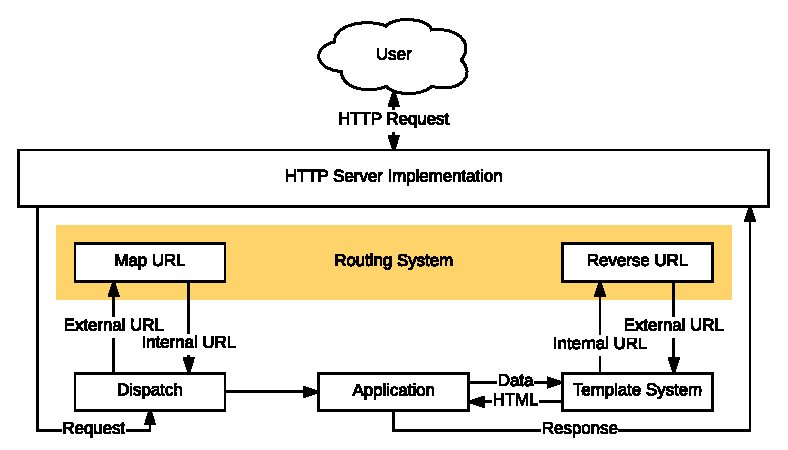
\includegraphics[width=\columnwidth]{request}
\end{frame}

\begin{frame}[fragile]
  \toptitle{Routing Definition}
\begin{lispcode}
aaaaaaa
\end{lispcode}
\end{frame}

\begin{frame}[fragile]
  \toptitle{Routing Example}
\begin{lispcode}
aaaaaaa
\end{lispcode}
\end{frame}

\begin{frame}
  \toptitle{Routing Advantages}
  \begin{itemize}
  \item aaaaaaa
  \end{itemize}
\end{frame}

\begin{frame}
  \toptitle{Environments}
\end{frame}

\begin{frame}
  \toptitle{Environment Access}
\end{frame}

\begin{frame}
  \toptitle{Environment Advantages}
\end{frame}

\begin{frame}
  \toptitle{Putting it All Together}
\end{frame}

\begin{frame}
  \toptitle{Existing Applications}
\end{frame}

\begin{frame}
  \toptitle{Resources}
\end{frame}

\begin{frame}
  \toptitle{Acknowledgements}
\end{frame}

\end{document}

%%% Local Variables:
%%% mode: latex
%%% TeX-master: t
%%% TeX-engine: luatex
%%% TeX-command-extra-options: "-shell-escape"
%%% End:
